\chapter{Конструкторская часть}

В данном разделе приведены схемы алгоритмов сортировок --- битонной, пирамидальной и вставками, приведено описание используемых типов данных.

\section{Требования к ПО}

К программе предъявлен ряд функциональных требований:
\begin{itemize}[label=---]
	\item должна иметь интерфейс для выбора действий;
	\item должна динамически выделять память под массив данных;
	\item должна замерять процессорное время работы реализации алгоритмов.
\end{itemize}

\section{Разработка алгоритмов}

На вход алгоритмов подаются указатель на массив $array$ и размер массива $n$ - целое положительное число.

На рисунках \ref{fig:insert} -- \ref{fig:comp_and_swap} представлены схемы алгоритмов сортировок, а именно сортировка вставками, пирамидальная сортировка и битонная сортировка.

\begin{figure}[h]
	\centering
	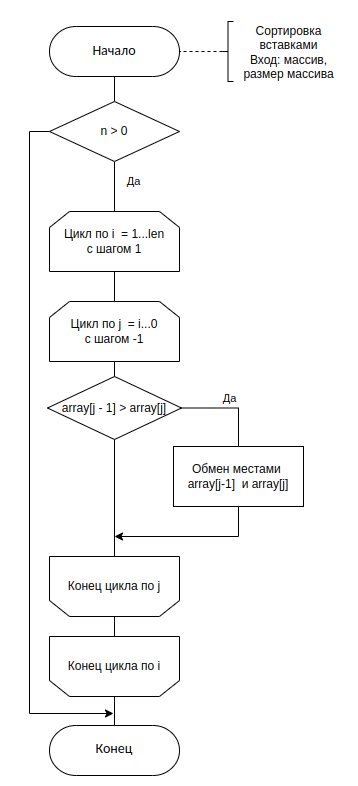
\includegraphics[height=0.8\textheight]{img/insert.png}
	\caption{Схема алгоритма сортировки вставками}
	\label{fig:insert}
\end{figure}

\clearpage

\begin{figure}[h]
	\centering
	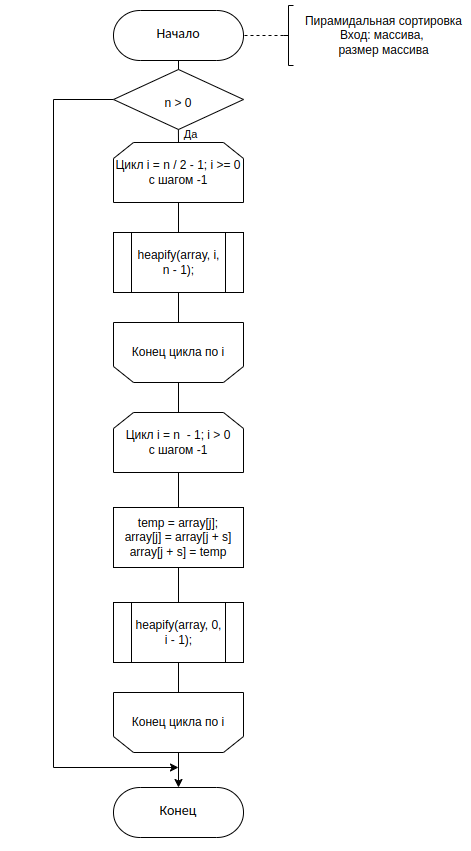
\includegraphics[height=0.8\textheight]{img/heap_1.png}
	\caption{Схема алгоритма пирамидальной сортировки}
	\label{fig:heap_1}
\end{figure}

\clearpage

\begin{figure}[h]
	\centering
	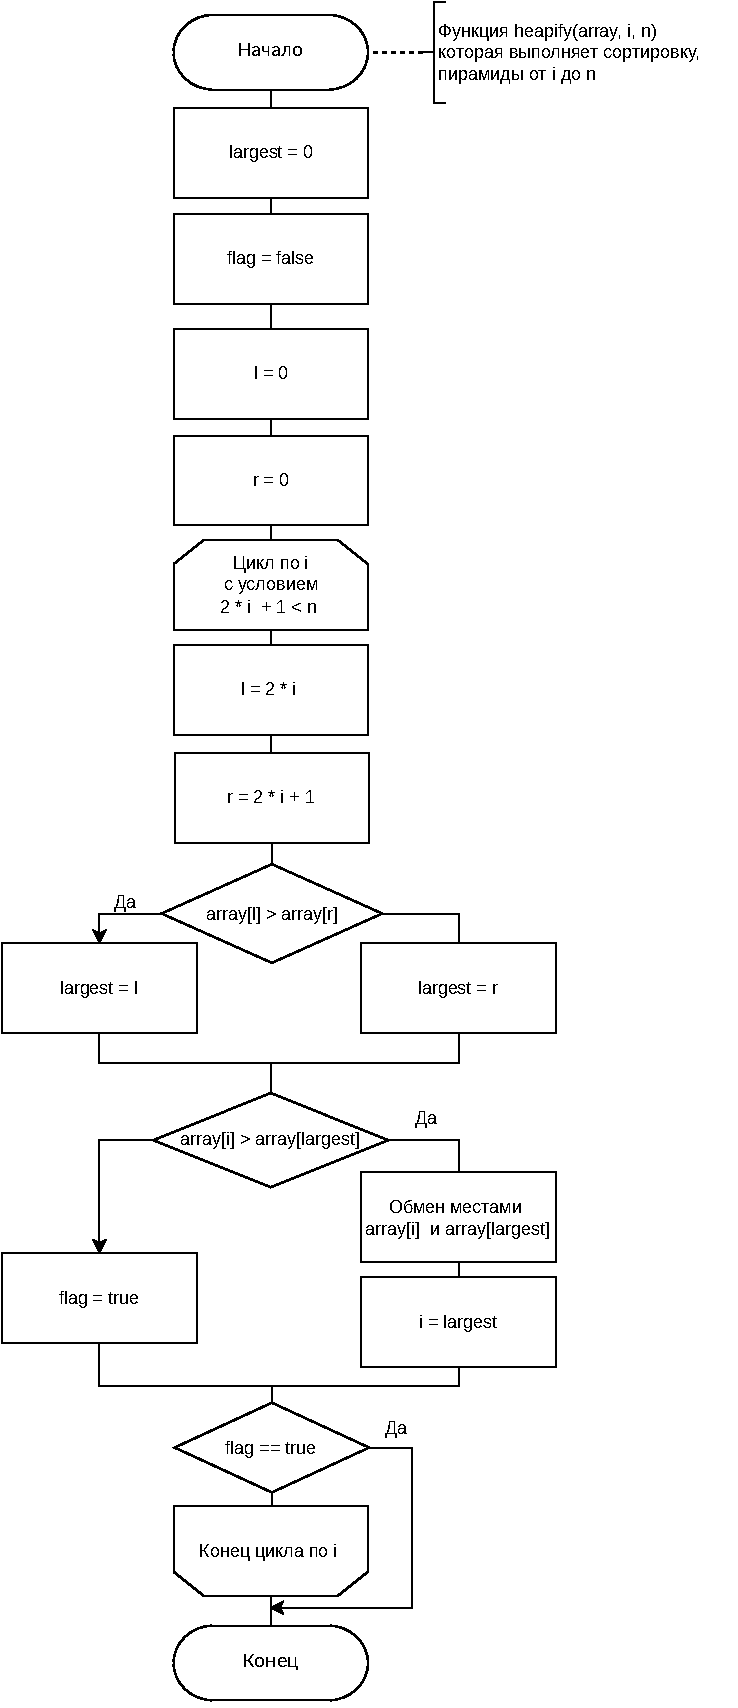
\includegraphics[height=0.8\textheight]{img/heap_2.pdf}
	\caption{Схема алгоритма функции heapify() для пирамидальной сортировки}
	\label{fig:heap_2}
\end{figure}

\clearpage

\begin{figure}[h]
	\centering
	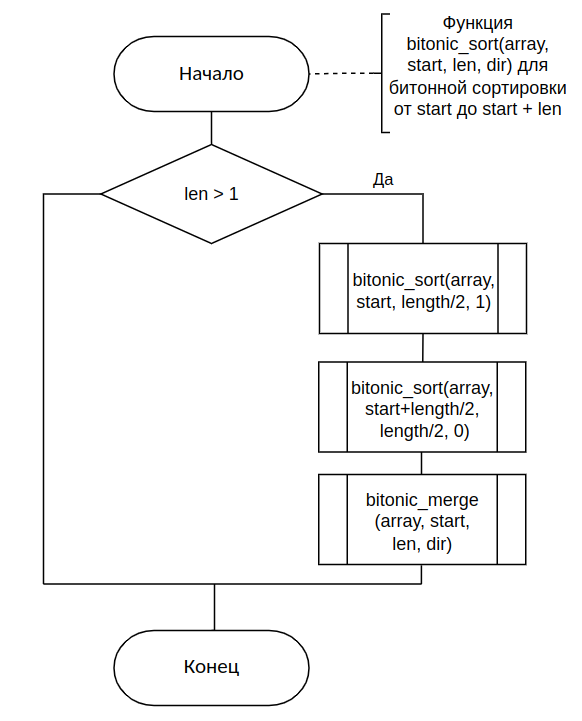
\includegraphics[height=0.7\textheight]{img/bitonic_2.png}
	\caption{Схема алгоритма функции bitonic\textunderscore sort() для битонной сортировки}
	\label{fig:bitonic_sort}
\end{figure}

\clearpage

\begin{figure}[h]
	\centering
	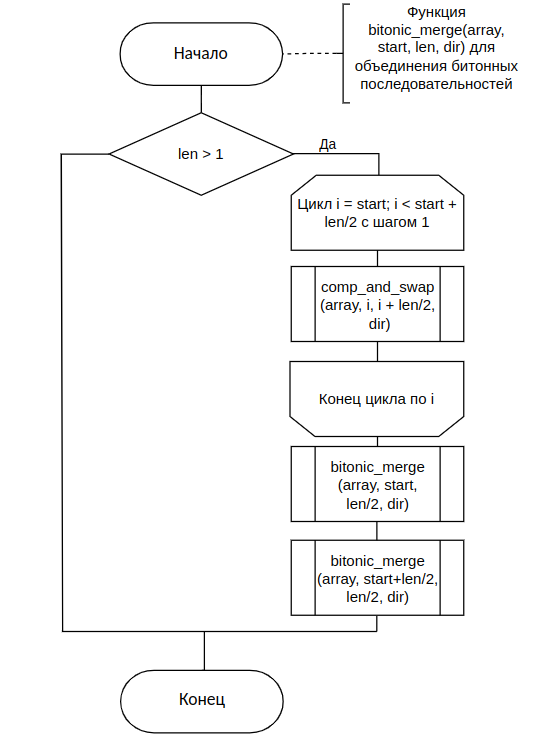
\includegraphics[height=0.8\textheight]{img/bitonic_3.png}
	\caption{Схема алгоритма функции bitonic\textunderscore merge() для битонной сортировки}
	\label{fig:bitonic_merge}
\end{figure}

\clearpage

\begin{figure}[h]
	\centering
	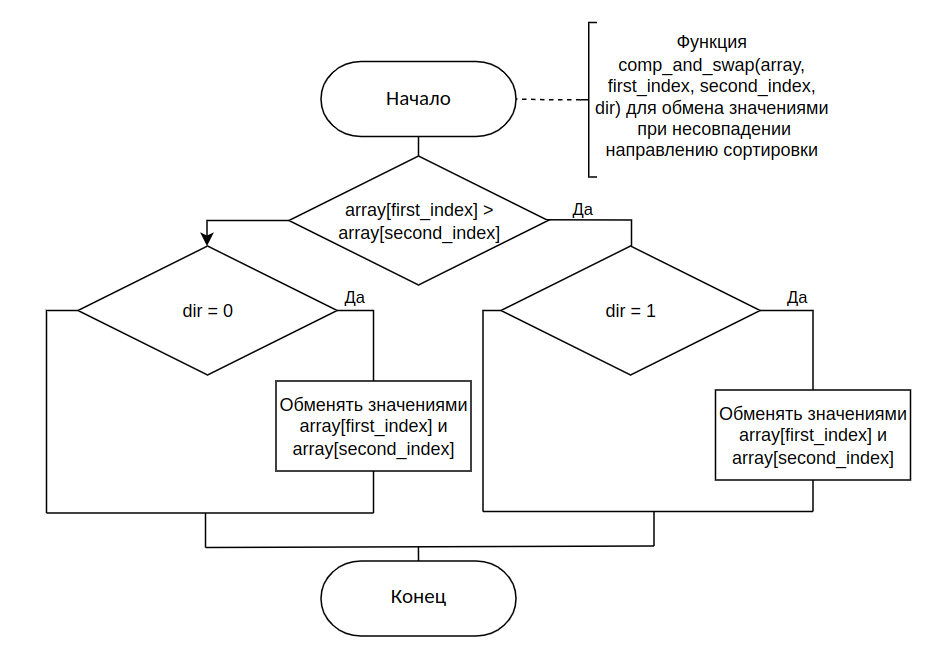
\includegraphics[height=0.4\textheight]{img/bitonic_4.png}
	\caption{Схема алгоритма функции comp\textunderscore and\textunderscore swap() для битонной сортировки}
	\label{fig:comp_and_swap}
\end{figure}

\clearpage

\section{Описание используемых типов данных}

При реализации алгоритмов будут использованы следующие структуры данных:

\begin{itemize}[label=---]
	\item указатель на массив типа $int *$;
	\item массив типа $int$;
	\item длина массива - целое число типа $size\_t$
\end{itemize}

\section{Модель для оценки трудоемкости}

Введем модель вычислений, которая потребуется для определения трудоемкости каждого отдельного взятого алгоритма сортировки.
\begin{enumerate}[label={\arabic*)}]
	\item Трудоемкость базовых операций:
	\begin{itemize}[label=---]
		\item для операций $+, -, =, +=, -=, ==, !=, <, >, <=, >=, [], ++,\\ {-}-,
			\&\&, >>, <<, ||, \&, |$
		трудоемкость равна 1;
		\item для операций $*, /, \%, *=, /=, \%=$
		трудоемкость равна 2.
	\end{itemize}
	\item Трудоемкость условного оператора:
	\begin{equation}
		\label{for:if}
		f_{if} = f_{\text{условия}} +
		\begin{cases}
			min(f_1, f_2), & \text{лучший случай},\\
			max(f_1, f_2), & \text{худший случай},
		\end{cases}
	\end{equation}
	где $f1$ и $f2$ - трудоемкости соответствующих ветвей условного оператора.
	\item Трудоемкость цикла:
	\begin{equation}
		\label{for:for}
		\begin{gathered}
			f_{for} = f_{\text{инициализация}} + f_{\text{сравнения}} + M_{\text{итераций}} \cdot (f_{\text{тело}} +\\
			+ f_{\text{инкремент}} + f_{\text{сравнения}}).
		\end{gathered}
	\end{equation}
	\item Трудоемкость передачи параметра в функции и возврат из функции равны 0.
\end{enumerate}

\section{Трудоемкость алгоритмов сортировки}

\subsection{Алгоритм сортировки вставками}

Трудоемкость в лучшем случае при отсортированном массиве.
Выведена в следующей формуле:
\begin{equation}
	\label{сomplexity:insert_best}
	\begin{gathered}
		f_{best} = 1 + (N - 1) \cdot 7 = 7 \cdot N - 6 = O(N).
	\end{gathered}
\end{equation}

Трудоемкость в худшем случае при отсортированном массиве в обратном порядке.
Выведена в следующей формуле:
\begin{equation}
	\label{сomplexity:insert_worst}
	\begin{gathered}
		f_{worst} = 1 + (N - 1) \cdot 8 + \frac{(N - 1) \cdot N \cdot 7}{2} = O(N^2).
	\end{gathered}
\end{equation}

\clearpage

\subsection{Алгоритм пирамидальной сортировки}

Трудоемкость в лучшем случае при отсортированном массиве.
Выведена в следующей формуле:
\begin{equation}
	\label{сomplexity:heap_best_t}
	\begin{gathered}
		f_{best} = 3 + 4 + \frac{N}{2} \cdot (2 + 1 + f_{heapify\_best}) + \\
		+ 3 + (N - 1)(2 + 2 + f_{swap} + 1 + f_{heapify\_best}).
	\end{gathered}
\end{equation}

Трудоемкость в худшем случае при отсортированном массиве в обратном порядке.
Выведена в следующей формуле:
\begin{equation}
	\label{сomplexity:heap_worst_t}
	\begin{gathered}
		f_{worst} = 3 + 4 + \frac{N}{2} \cdot (2 + 1 + f_{heapify\_worst}) + \\
		+ 3 + (N - 1)(2 + 2 + f_{swap} + 1 + f_{heapify\_worst}).
	\end{gathered}
\end{equation}

Трудоемкость перестановки элементов будет равна результату вычисления следующей формулы:
\begin{equation}
	\label{сomplexity:swap}
	f_{swap} = 1 + 1 + 1 = 3.
\end{equation}

Часть трудоемкости пирамидальной сортировки содержится в функции heapify(), формула для ее расчета:
\begin{equation}
	\label{сomplexity:heapify}
	f_{heapify} = 5 + log N \cdot (5 + 3 + 4 + 1 +
	\begin{cases}
		1, \\
		3 + \begin{cases}
			1, \\
			1,
		\end{cases},
	\end{cases} + 3 +
	\begin{cases}
		1, \\
		4,
	\end{cases})
\end{equation}

Исходя из формулы (\ref{сomplexity:heapify}) были выведены лучший (\ref{сomplexity:heapify_best}) и худший (\ref{сomplexity:heapify_worst}) случаи функции heapify:
\begin{equation}
	\label{сomplexity:heapify_best}
	f_{heapify\_best} = 5 + log N \cdot (5 + 3 + 4 + 2 + 4) = 5 + 17 \cdot log N = O(log N)
\end{equation}
\begin{equation}
	\label{сomplexity:heapify_worst}
	f_{heapify\_worst} = 5 + log N \cdot (5 + 3 + 4 + 5 + 7) = 5 + 24 \cdot log N = O(log N)
\end{equation}

Исходя из выведенных выше трудоемкостей, можно вычислить трудоемкость лучшего и худшего случая по формулам:

\begin{equation}
	\label{сomplexity:heap_best_p}
	\begin{gathered}
		f_{best} = 7 + \frac{N}{2} \cdot (3 + 5 + 17 \cdot log N) + 3 + (N - 1) \cdot (5 + 3 + \\
		+ 5 + 17 \cdot log N) = 23N + 27N \cdot log N - 13 \cdot log N - 3 =\\
		= O(N \cdot log N),
	\end{gathered}
\end{equation}

\begin{equation}
	\label{сomplexity:heap_worst_p}
	\begin{gathered}
		f_{worst} = 7 + \frac{N}{2} \cdot (3 + 5 + 24 \cdot log N) + 3 + (N - 1) \cdot (5 + 3 + \\
		+ 5 + 24 \cdot log N) = 23N + 36N \cdot log N - 24 \cdot log N - 3 =\\
		= O(N \cdot log N).
	\end{gathered}
\end{equation}

Таким образов из выведенных в формулах (\ref{сomplexity:heap_best_p}) и (\ref{сomplexity:heap_worst_p}) результатов можно понять, что лучший и худший случай имеют трудоемкость $O(N \cdot log N)$.

\subsection{Алгоритм битонной сортировки}
% Количество сравнений на каждом слиянии - N/2,
% потому количество обменов на каждом шаге ограничено сверху N/2.
% Трудоёмкость каждого обмена - 7.
% Трудоёмкость каждого сравнения - 4.
% Всего шагов - log(N) * (log(N) + 1) / 2.

% 239 страница в кнуте

Пусть a - среднее количество обменов на каждом шаге, причем $0 < a < \frac{N}{2}$, тогда итоговая трудоемкость алгоритма:
\begin{equation}
	\label{сomplexity:bitonic}
	\begin{gathered}
		f_{best} = \frac{log{N} \cdot (log(N) + 1)}{2} \cdot (\frac{N}{2} \cdot 4 + a \cdot 7) = O((log N)^2\cdot N)
	\end{gathered}
\end{equation}

Можно заметить, что результирующая трудоемкость не зависит от a, следовательно лучший и худший случай имеют одинаковую трудоемкость $O((log N)^2\cdot N)$.
\section*{Вывод}

В данном разделе на основе теоретических данных были построены схемы требуемых алгоритмов, выбраны используемые типы данных.
Для каждого алгоритма сортировки были выведены трудоемкости худшего и лучшего случаев.
